\chapter{Temporal Certificates and Graceful Degradation}
\label{ch:temporal-certificates-graceful-degradation}

\section{Certificate horizon as a runtime object}
ORIUS certificates are temporal objects, not merely one-step labels. A certificate has a
validity horizon, an expiration condition, and a bounded interpretation under worsening
observation. This matters because degraded telemetry can remain acceptable for one step and
become unacceptable only a short time later. The temporal question is therefore not
``safe or unsafe forever,'' but ``how long does the runtime have before the current
certificate no longer justifies release?''

\section{Expiration, half-life, and safe-hold}
The dissertation treats horizon and half-life conservatively. The current evidence is
strongest for bounded expiration and safe-hold semantics under blackout-style degradation.
That is the right level of claim: certificate time is measurable and governable, but it is
not yet promoted into a universal law of every plant and every sensor regime.

\begin{figure}[htbp]
\centering
\IfFileExists{reports/publication/fig_blackout_halflife.png}{%
\includegraphics[width=0.80\textwidth]{reports/publication/fig_blackout_halflife.png}%
}{%
\includegraphics[width=0.80\textwidth]{../reports/publication/fig_blackout_halflife.png}%
}
\caption{Blackout half-life surface used to motivate certificate expiration, bounded safe-hold, and temporal intervention discipline.}
\label{fig:blackout-half-life}
\end{figure}

\section{Graceful degradation policies}
When no full-quality control action remains justified, ORIUS benchmarks degradation
policies explicitly rather than treating them as informal emergency behavior. This is the
runtime-assurance connection in practice: the system needs a governed way to do less,
safer, and more explainably when observation quality collapses.

\begin{figure}[htbp]
\centering
\IfFileExists{reports/publication/fig_graceful_four_policies.png}{%
\includegraphics[width=0.86\textwidth]{reports/publication/fig_graceful_four_policies.png}%
}{%
\includegraphics[width=0.86\textwidth]{../reports/publication/fig_graceful_four_policies.png}%
}
\caption{Four-policy graceful degradation comparison. The dissertation uses this family to treat fallback quality as a benchmarked layer instead of an unexamined emergency default.}
\label{fig:graceful-four-policies}
\end{figure}

\section{Bounded claim}
The temporal chapter supports a bounded but important claim: certificate time and graceful
degradation can be benchmarked and governed as part of the same runtime object as repair
and fallback. It does not claim a universal optimal degradation policy, and it does not
erase the domain-specific obligations that remain tied to the parity matrix.
